\documentclass[11pt,a4paper]{article}
% ── Typography ────────────────────────────────────────────────────────────────
\usepackage[margin=2.5cm]{geometry}
\usepackage[utf8]{inputenc}
\usepackage[T1]{fontenc}
\usepackage{lmodern}
\usepackage{microtype}
% ── Graphics ─────────────────────────────────────────────────────────────────
\usepackage{xcolor}
\usepackage{tikz}
\usepackage{pgfplots}
\pgfplotsset{compat=1.18}
\usetikzlibrary{shapes.geometric, arrows.meta, positioning, fit, backgrounds,
                decorations.pathreplacing, calc}
% ── Tables ───────────────────────────────────────────────────────────────────
\usepackage{booktabs}
\usepackage{array}
\usepackage{colortbl}
\usepackage{multirow}
% ── Document ─────────────────────────────────────────────────────────────────
\usepackage{listings}
\usepackage{hyperref}
\usepackage{fancyhdr}
\usepackage{amsmath}
\usepackage{pifont}
\usepackage{enumitem}

% ── Colours ───────────────────────────────────────────────────────────────────
\definecolor{fpgablue}{RGB}{13,71,161}
\definecolor{fpgalight}{RGB}{187,222,251}
\definecolor{hostgreen}{RGB}{27,94,32}
\definecolor{hostlight}{RGB}{200,230,201}
\definecolor{ibkrorange}{RGB}{200,80,0}
\definecolor{ibkrlight}{RGB}{255,224,178}
\definecolor{sigred}{RGB}{183,28,28}
\definecolor{codegray}{RGB}{248,248,248}
\definecolor{arrowgray}{RGB}{80,80,80}
\definecolor{fixgreen}{RGB}{76,175,80}
\definecolor{awsyellow}{RGB}{200,120,0}
\definecolor{awslight}{RGB}{255,243,191}
\definecolor{noteyellow}{RGB}{255,249,196}
\definecolor{noteborder}{RGB}{255,193,7}

\newcommand{\cmark}{\textcolor{fixgreen}{\ding{51}}}
\newcommand{\pmark}{\textcolor{gray}{\ding{109}}}
\newcommand{\todo}{\textcolor{gray!70}{\textit{[measured on F1]}}}

% ── TikZ styles ───────────────────────────────────────────────────────────────
\tikzset{
  block/.style={rectangle, rounded corners=4pt, minimum width=2.8cm,
    minimum height=0.9cm, text centered, draw, font=\small\bfseries,
    text width=2.6cm},
  fpgablock/.style={block, fill=fpgalight, draw=fpgablue, text=fpgablue},
  hostblock/.style={block, fill=hostlight, draw=hostgreen, text=hostgreen},
  ibkrblock/.style={block, fill=ibkrlight, draw=ibkrorange, text=ibkrorange},
  awsblock/.style={block, fill=awslight, draw=awsyellow, text=awsyellow},
  riskblock/.style={block, fill=sigred!8, draw=sigred!60, text=sigred,
                    minimum width=5.5cm, text width=5.3cm, minimum height=0.6cm,
                    font=\scriptsize},
  arrow/.style={-{Stealth[length=6pt]}, thick, color=arrowgray},
  fatarrow/.style={-{Stealth[length=8pt]}, line width=2pt, color=fpgablue},
  slowarrow/.style={-{Stealth[length=8pt]}, line width=2pt, color=ibkrorange},
  dashbox/.style={rectangle, rounded corners=6pt, dashed, inner sep=10pt},
}

% ── Page style ────────────────────────────────────────────────────────────────
\pagestyle{fancy}
\fancyhf{}
\rhead{\small\textcolor{fpgablue}{FPGA Tick-to-Trade}}
\lhead{\small Part 3: Integration, Deployment \& Results}
\cfoot{\small\thepage}
\renewcommand{\headrulewidth}{0.5pt}

\hypersetup{colorlinks=true, linkcolor=fpgablue, urlcolor=fpgablue,
            pdftitle={FPGA Tick-to-Trade Part 3}}

\lstset{
  backgroundcolor=\color{codegray}, basicstyle=\ttfamily\footnotesize,
  keywordstyle=\color{fpgablue}\bfseries, commentstyle=\color{gray}\itshape,
  breaklines=true, frame=single, rulecolor=\color{gray!40},
  numbers=left, numberstyle=\tiny\color{gray},
  xleftmargin=1.5em, xrightmargin=0.5em,
}

% ─────────────────────────────────────────────────────────────────────────────
\begin{document}

\begin{titlepage}
\begin{tikzpicture}[remember picture, overlay]
  \fill[fpgablue] (current page.north west)
    rectangle ([yshift=-7cm]current page.north east);
  \foreach \x in {0,1,...,30} {
    \draw[white, opacity=0.04, very thin]
      ([xshift=\x*0.7cm]current page.north west)
      -- ([xshift=\x*0.7cm,yshift=-7cm]current page.north west);
  }
  \foreach \y in {0,...,10} {
    \draw[white, opacity=0.04, very thin]
      ([yshift=-\y*0.7cm]current page.north west)
      -- ([yshift=-\y*0.7cm]current page.north east);
  }
  \node[text=white, font=\fontsize{28}{34}\selectfont\bfseries, anchor=north west]
    at ([xshift=2.5cm, yshift=-2.0cm]current page.north west)
    {FPGA Tick-to-Trade};
  \node[text=white!85, font=\Large, anchor=north west]
    at ([xshift=2.5cm, yshift=-3.6cm]current page.north west)
    {Part 3 \textemdash\ Integration, Deployment \& Results};
  \node[text=white!60, font=\normalsize, anchor=north west]
    at ([xshift=2.5cm, yshift=-5.0cm]current page.north west)
    {Abhishek\ \ $\cdot$\ \ June 2026\ \ $\cdot$\ \ Updated as milestones complete};
  \node[text=white!50, font=\small\itshape, anchor=north west]
    at ([xshift=2.5cm, yshift=-6.0cm]current page.north west)
    {AWS F1 deployment $\cdot$ IBKR paper account $\cdot$ latency measurement};
\end{tikzpicture}
\vspace*{8cm}
\tableofcontents
\end{titlepage}

% ─────────────────────────────────────────────────────────────────────────────
\section{Why Latency Numbers Matter}

\subsection{Market Microstructure: The Speed Premium}

In a competitive market, the ``speed premium'' is real and measurable.
Consider a simple scenario: a large market-moving order arrives on one exchange.
An HFT system that detects it in hardware within 100\,ns can immediately
re-quote on correlated instruments before slower participants react.
The window for this opportunity is often 1--50\,$\mu$s.

\begin{center}
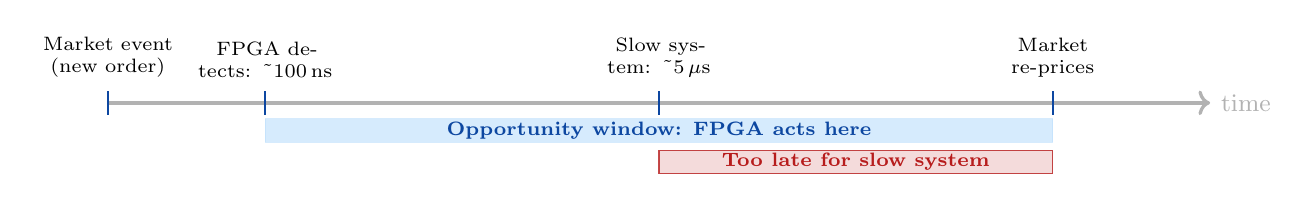
\begin{tikzpicture}[font=\small]
  % Timeline
  \draw[very thick, gray!60, ->] (0,0) -- (14,0) node[right] {time};
  \draw[thick, fpgablue] (0,-0.15) -- (0,0.15);
  \node[font=\scriptsize, align=center, text width=1.8cm, above=0.2cm] at (0,0)
    {Market event (new order)};
  \draw[thick, fpgablue] (2,-0.15) -- (2,0.15);
  \node[font=\scriptsize, align=center, text width=2cm, above=0.2cm] at (2,0)
    {FPGA detects: \textasciitilde{}100\,ns};
  \draw[thick, fpgablue] (7,-0.15) -- (7,0.15);
  \node[font=\scriptsize, align=center, text width=2cm, above=0.2cm] at (7,0)
    {Slow system: \textasciitilde{}5\,$\mu$s};
  \draw[thick, fpgablue] (12,-0.15) -- (12,0.15);
  \node[font=\scriptsize, align=center, text width=1.8cm, above=0.2cm] at (12,0)
    {Market re-prices};
  % Opportunity window
  \draw[fpgalight, fill=fpgalight, opacity=0.6]
    (2,-0.5) rectangle (12,-0.2);
  \node[font=\scriptsize\bfseries, fpgablue] at (7,-0.35)
    {Opportunity window: FPGA acts here};
  \draw[sigred, fill=sigred!20, opacity=0.8]
    (7,-0.9) rectangle (12,-0.6);
  \node[font=\scriptsize\bfseries, sigred] at (9.5,-0.75)
    {Too late for slow system};
\end{tikzpicture}
\end{center}

\subsection{p99 Tail Latency: Why Median Is Not Enough}

A CPU-based system might have a median (p50) latency of 2\,$\mu$s, but the
99th percentile (p99) can be 100--1000$\times$ higher due to OS scheduler
jitter, CPU cache misses, and interrupt handling. In HFT, the p99 latency
determines how often your system \emph{misses} its window --- even if it
wins most of the time, losing 1\% of the time due to jitter can dominate profits.

An FPGA pipeline eliminates this variance entirely. With a constant $N$-cycle
pipeline, p1 = p50 = p99 = $N \times T_{clk}$.

% ─────────────────────────────────────────────────────────────────────────────
\section{Full Integration Test}

The full integration test drives \texttt{tick\_to\_trade\_top} --- the complete
wired pipeline --- with a synthetic ITCH scenario designed to trigger a BUY signal.

\begin{center}
\begin{tikzpicture}[node distance=0.6cm and 0.7cm]

  %% Left column: flow
  \node[block, fill=noteyellow, draw=noteborder,
        minimum width=4.5cm, text width=4.3cm]
    (synth) {\texttt{synth\_itch.py}\\Build 4-message scenario};

  \node[fpgablock, below=0.7cm of synth,
        minimum width=4.5cm, text width=4.3cm]
    (top) {\texttt{tick\_to\_trade\_top.sv}\\Full pipeline DUT};

  \node[fpgablock, right=2.5cm of top, minimum width=3.2cm, text width=3.0cm]
    (lat) {\texttt{latency\_counter}\\cycle histogram};

  \node[block, fill=noteyellow, draw=noteborder,
        below=0.7cm of top, minimum width=4.5cm, text width=4.3cm]
    (check) {Assert:\\decision fires?\\\texttt{action}=BUY? price correct?\\latency in range?};

  \draw[fatarrow] (synth) -- (top);
  \draw[arrow, dashed, fpgablue] (top.east) -- (lat.west)
    node[midway, above, font=\scriptsize]{\texttt{msg\_start}};
  \draw[arrow, dashed, fpgablue] ([yshift=-0.3cm]top.east) -- ([yshift=-0.3cm]lat.west)
    node[midway, below, font=\scriptsize]{\texttt{decision\_valid}};
  \draw[fatarrow] (top) -- (check);
  \draw[fatarrow] (lat.south) |- (check.east);

  %% Right column: scenario
  \node[font=\scriptsize\bfseries, fpgablue]
    at (10.5, 0.3) {Test scenario:};

  \node[fpgablock, minimum width=5.0cm, text width=4.8cm, minimum height=0.65cm,
        font=\scriptsize] (m1) at (10.5, -0.5)
    {msg 1: Add bid \$149.99, 100 shares};
  \node[fpgablock, minimum width=5.0cm, text width=4.8cm, minimum height=0.65cm,
        font=\scriptsize] (m2) at (10.5, -1.3)
    {msg 2: Add ask \$150.01, 60 shares};
  \node[fpgablock, minimum width=5.0cm, text width=4.8cm, minimum height=0.65cm,
        font=\scriptsize] (m3) at (10.5, -2.1)
    {msg 3: Add bid \$149.99, 200 shares};
  \node[fpgablock, minimum width=5.0cm, text width=4.8cm, minimum height=0.65cm,
        font=\scriptsize] (m4) at (10.5, -2.9)
    {msg 4: Add bid \$149.99, 150 shares};

  \node[block, fill=fixgreen!15, draw=fixgreen, text=hostgreen,
        minimum width=5.0cm, text width=4.8cm, minimum height=0.75cm,
        font=\scriptsize\bfseries] (dec) at (10.5, -3.9)
    {BUY signal fires! bid=450, ask=60\\$450{\times}10 = 4500 > 15{\times}60 = 900$\ \cmark};

  \draw[arrow] (m1) -- (m2); \draw[arrow] (m2) -- (m3);
  \draw[arrow] (m3) -- (m4); \draw[fatarrow] (m4) -- (dec);
\end{tikzpicture}
\end{center}

% ─────────────────────────────────────────────────────────────────────────────
\section{Host Software}

\subsection{Pre-Trade Risk: SEC Rule 15c3-5}

SEC Rule 15c3-5 (the ``Market Access Rule'') requires broker-dealers to have
\textbf{risk controls that prevent erroneous orders} before they reach the market.
These controls must be implemented in a way that catches problems even if the
trading algorithm malfunctions.

The rule specifically requires:
\begin{itemize}[itemsep=2pt]
  \item \textbf{Financial exposure limits}: maximum order value, maximum position
  \item \textbf{Erroneous order prevention}: fat-finger filters (price bands)
  \item \textbf{Order rate limits}: prevent runaway order loops
  \item \textbf{Capital thresholds}: don't exceed available capital
\end{itemize}

In this project, the risk checks are implemented in \texttt{risk\_guard.py}
on the EC2 host (software layer) and will be duplicated in hardware
(\texttt{risk\_check.sv}) in Milestone 2.

\subsection{\texttt{risk\_guard.py} --- Five Checks}

\begin{center}
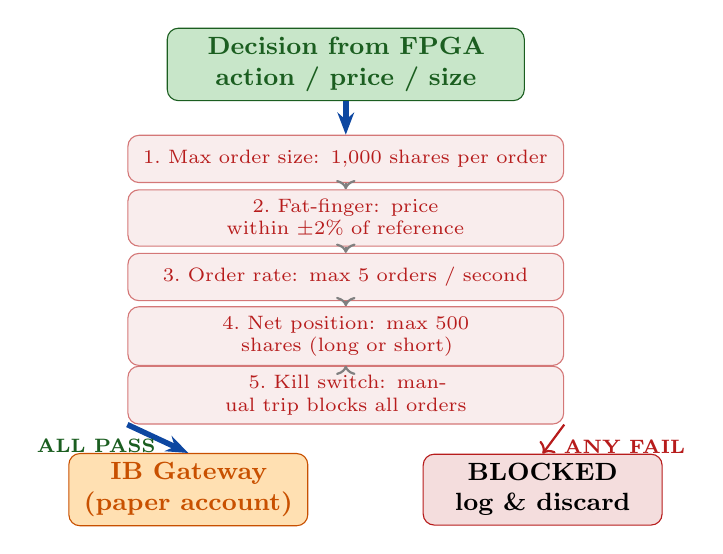
\begin{tikzpicture}[node distance=0.35cm]
  % Input
  \node[hostblock, minimum width=4.5cm, text width=4.3cm] (inp) at (0,0)
    {Decision from FPGA\\action / price / size};

  % Five risk check boxes (explicit absolute positions)
  \node[riskblock] (r1) at (0, -1.2)
    {1.\ Max order size: 1{,}000 shares per order};
  \node[riskblock] (r2) at (0, -1.95)
    {2.\ Fat-finger: price within $\pm$2\% of reference};
  \node[riskblock] (r3) at (0, -2.7)
    {3.\ Order rate: max 5 orders / second};
  \node[riskblock] (r4) at (0, -3.45)
    {4.\ Net position: max 500 shares (long or short)};
  \node[riskblock] (r5) at (0, -4.2)
    {5.\ Kill switch: manual trip blocks all orders};

  % Outputs
  \node[ibkrblock, minimum width=3.0cm, text width=2.8cm] (gw) at (-2.0, -5.4)
    {IB Gateway\\(paper account)};
  \node[block, fill=sigred!15, draw=sigred, minimum width=3.0cm, text width=2.8cm]
    (blk) at (2.5, -5.4)
    {BLOCKED\\log \& discard};

  % Arrows
  \draw[fatarrow] (inp.south) -- (r1.north);
  \draw[arrow, gray, ->] (r1) -- (r2); \draw[arrow, gray, ->] (r2) -- (r3);
  \draw[arrow, gray, ->] (r3) -- (r4); \draw[arrow, gray, ->] (r4) -- (r5);
  \draw[fatarrow] (r5.south west) -- (gw.north)
    node[near end, left=2pt, font=\scriptsize\bfseries, hostgreen]{ALL PASS};
  \draw[arrow, sigred, ->] (r5.south east) -- (blk.north)
    node[near end, right=2pt, font=\scriptsize\bfseries, sigred]{ANY FAIL};
\end{tikzpicture}
\end{center}

\subsection{IBKR Bridge: \texttt{ibkr\_bridge.py}}

\begin{center}
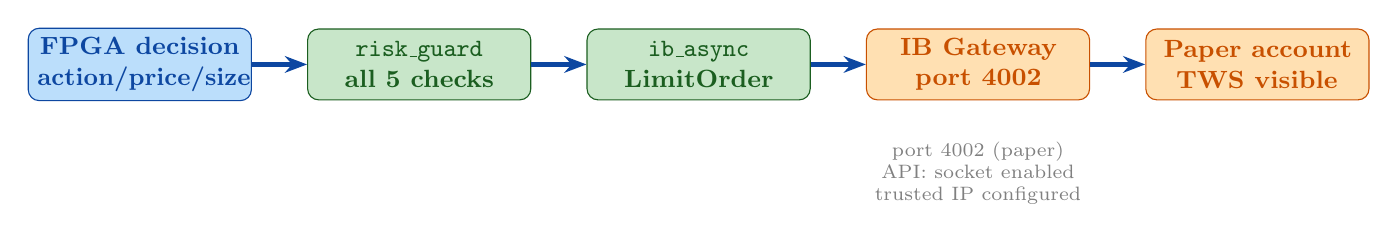
\begin{tikzpicture}[node distance=0.4cm and 0.9cm]
  \node[fpgablock, minimum width=2.8cm, text width=2.6cm]
    (fpga) {FPGA decision\\action/price/size};
  \node[hostblock, right=0.7cm of fpga, minimum width=2.8cm, text width=2.6cm]
    (risk) {\texttt{risk\_guard}\\all 5 checks};
  \node[hostblock, right=0.7cm of risk, minimum width=2.8cm, text width=2.6cm]
    (ib) {\texttt{ib\_async}\\LimitOrder};
  \node[ibkrblock, right=0.7cm of ib, minimum width=2.8cm, text width=2.6cm]
    (gw) {IB Gateway\\port 4002};
  \node[ibkrblock, right=0.7cm of gw, minimum width=2.8cm, text width=2.6cm]
    (acc) {Paper account\\TWS visible};

  \draw[fatarrow] (fpga) -- (risk);
  \draw[fatarrow] (risk) -- (ib);
  \draw[fatarrow] (ib)   -- (gw);
  \draw[fatarrow] (gw)   -- (acc);

  \node[font=\scriptsize, gray, below=0.4cm of gw, align=center]
    {port 4002 (paper)\\API: socket enabled\\trusted IP configured};
\end{tikzpicture}
\end{center}

\subsection{Dry-Run Testing (No IBKR Required)}

Before connecting to any account, the bridge can be tested in dry-run mode:

\begin{lstlisting}[language=Python, caption={Dry-run test of ibkr\_bridge.py}]
# No IBKR connection needed
python host/ibkr_bridge.py --demo

# Expected output:
INFO  DRY-RUN mode -- no real connection
INFO  ORDER  BUY  100 @ $150.0000 -> risk PASS
INFO  DRY-RUN: would place BUY  100 @ 150.0000
INFO  ORDER  SELL 100 @ $150.0500 -> risk PASS
INFO  DRY-RUN: would place SELL 100 @ 150.0500
\end{lstlisting}

% ─────────────────────────────────────────────────────────────────────────────
\section{AWS F1 Deployment}

\subsection{What Is AWS F1?}

AWS F1 instances are EC2 virtual machines with a \textbf{real Xilinx UltraScale+
VU9P FPGA} physically attached via PCIe. The FPGA connects to:

\begin{itemize}[itemsep=2pt]
  \item The EC2 x86 host CPU via \textbf{PCIe Gen3 $\times$16} (DMA for data transfer)
  \item Two \textbf{400\,Gb/s DRAM banks} directly on the FPGA board
  \item A \textbf{25\,Gb/s Ethernet port} connected directly to the FPGA
    Programmable Logic (PL) --- critical for wire-to-wire latency measurement
\end{itemize}

\begin{center}
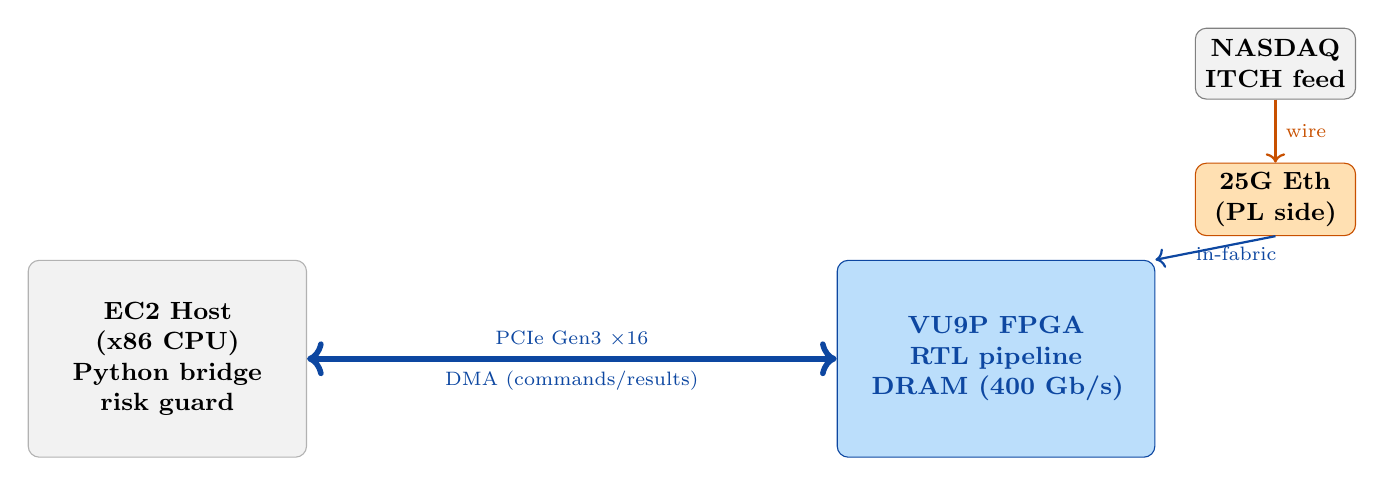
\begin{tikzpicture}[font=\small, node distance=0.5cm and 0.8cm]
  \node[block, fill=gray!10, draw=gray!60,
        minimum width=3.5cm, text width=3.3cm, minimum height=2.5cm]
    (ec2) at (0,0) {EC2 Host\\(x86 CPU)\\Python bridge\\risk guard};

  \node[fpgablock, right=2.5cm of ec2,
        minimum width=4cm, text width=3.8cm, minimum height=2.5cm]
    (fpga) at (6,0) {VU9P FPGA\\RTL pipeline\\DRAM (400 Gb/s)};

  \node[block, fill=ibkrlight, draw=ibkrorange,
        minimum width=2cm, above right=0.3cm and 0.5cm of fpga, text width=1.8cm]
    (eth) {25G Eth\\(PL side)};

  \node[block, fill=gray!10, draw=gray, minimum width=2cm,
        above=0.8cm of eth, text width=1.8cm]
    (net) {NASDAQ\\ITCH feed};

  \draw[fatarrow, <->] (ec2.east) -- (fpga.west)
    node[midway, above, font=\scriptsize]{PCIe Gen3 $\times$16}
    node[midway, below, font=\scriptsize]{DMA (commands/results)};
  \draw[arrow, ibkrorange, ->] (net) -- (eth)
    node[midway, right, font=\scriptsize]{wire};
  \draw[arrow, fpgablue, ->] (eth.south) -- (fpga.north east)
    node[near end, right, font=\scriptsize]{in-fabric};
\end{tikzpicture}
\end{center}

\subsection{F1 vs Local Development: Cost Breakdown}

\begin{center}
\small
\begin{tabular}{l l r}
\toprule
\textbf{Activity} & \textbf{Where} & \textbf{Cost} \\
\midrule
All RTL simulation (unlimited iterations) & Local VM: QuestaSim & Free \\
Synthesis sanity check                    & AWS FPGA Dev AMI (EC2) & \textasciitilde\$0.10/hr \\
Full AFI bitstream build (one-time)       & AWS EC2 (Vivado \textasciitilde{}2 hrs) & \textasciitilde\$2--3 total \\
Hardware test on real VU9P FPGA           & AWS F1 f1.2xlarge & \$1.65/hr \\
\midrule
\multicolumn{2}{l}{\bfseries Total estimated cost (Milestone 1 hardware phase)} & \textbf{\textasciitilde\$10--15} \\
\bottomrule
\end{tabular}
\end{center}

\subsection{AFI Build Flow}

An \textbf{Amazon FPGA Image (AFI)} is the F1 equivalent of a bitstream.
AWS compiles your RTL into an AFI using Vivado on their infrastructure; you
then load the AFI onto the FPGA without needing to manage the full synthesis flow locally.

\begin{center}
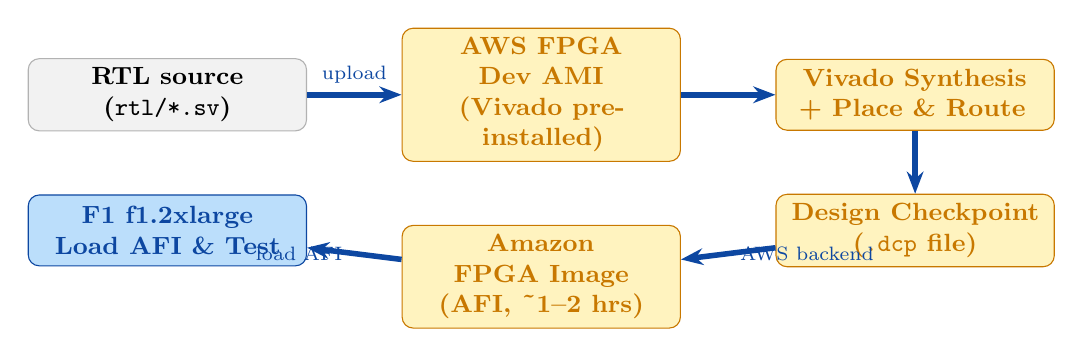
\begin{tikzpicture}[node distance=0.5cm and 0.7cm]
  \node[block, fill=gray!10, draw=gray!60, minimum width=3.5cm, text width=3.3cm]
    (rtl) {RTL source\\(\texttt{rtl/*.sv})};

  \node[awsblock, right=1.2cm of rtl, minimum width=3.5cm, text width=3.3cm]
    (ami) {AWS FPGA Dev AMI\\(Vivado pre-installed)};

  \node[awsblock, right=1.2cm of ami, minimum width=3.5cm, text width=3.3cm]
    (synth) {Vivado Synthesis\\+ Place \& Route};

  \node[awsblock, below=0.8cm of synth, minimum width=3.5cm, text width=3.3cm]
    (dcp) {Design Checkpoint\\(\texttt{.dcp} file)};

  \node[awsblock, below=0.8cm of ami, minimum width=3.5cm, text width=3.3cm]
    (afi) {Amazon FPGA Image\\(AFI, \textasciitilde{}1--2 hrs)};

  \node[fpgablock, below=0.8cm of rtl, minimum width=3.5cm, text width=3.3cm]
    (f1) {F1 f1.2xlarge\\Load AFI \& Test};

  \draw[fatarrow] (rtl)   -- (ami)   node[midway,above,font=\scriptsize]{upload};
  \draw[fatarrow] (ami)   -- (synth);
  \draw[fatarrow] (synth) -- (dcp);
  \draw[fatarrow] (dcp)   -- (afi)   node[midway,right,font=\scriptsize]{AWS backend};
  \draw[fatarrow] (afi)   -- (f1)    node[midway,left,font=\scriptsize]{load AFI};
\end{tikzpicture}
\end{center}

% ─────────────────────────────────────────────────────────────────────────────
\section{Latency Results}

\subsection{FPGA Pipeline Latency (Hardware-Measured)}

\begin{center}
\small
\begin{tabular}{l r}
\toprule
\textbf{Metric} & \textbf{Value} \\
\midrule
Clock frequency           & 200\,MHz \\
Clock period              & 5\,ns \\
Pipeline depth (first byte $\rightarrow$ decision) & \todo\ cycles \\
Tick-to-trade latency p50 & \todo\ ns \\
Tick-to-trade latency p99 & \todo\ ns \\
Throughput                & \todo\ M\,msgs/sec \\
\bottomrule
\end{tabular}
\end{center}

\subsection{IBKR Software Path (End-to-End)}

\begin{center}
\small
\begin{tabular}{l r}
\toprule
\textbf{Metric} & \textbf{Value} \\
\midrule
Average order round-trip  & \textasciitilde30\,ms (typical) \\
p50                       & \todo\ ms \\
p99                       & \todo\ ms \\
\bottomrule
\end{tabular}
\end{center}

\subsection{The Money-Shot: Latency Comparison Chart}

\begin{center}
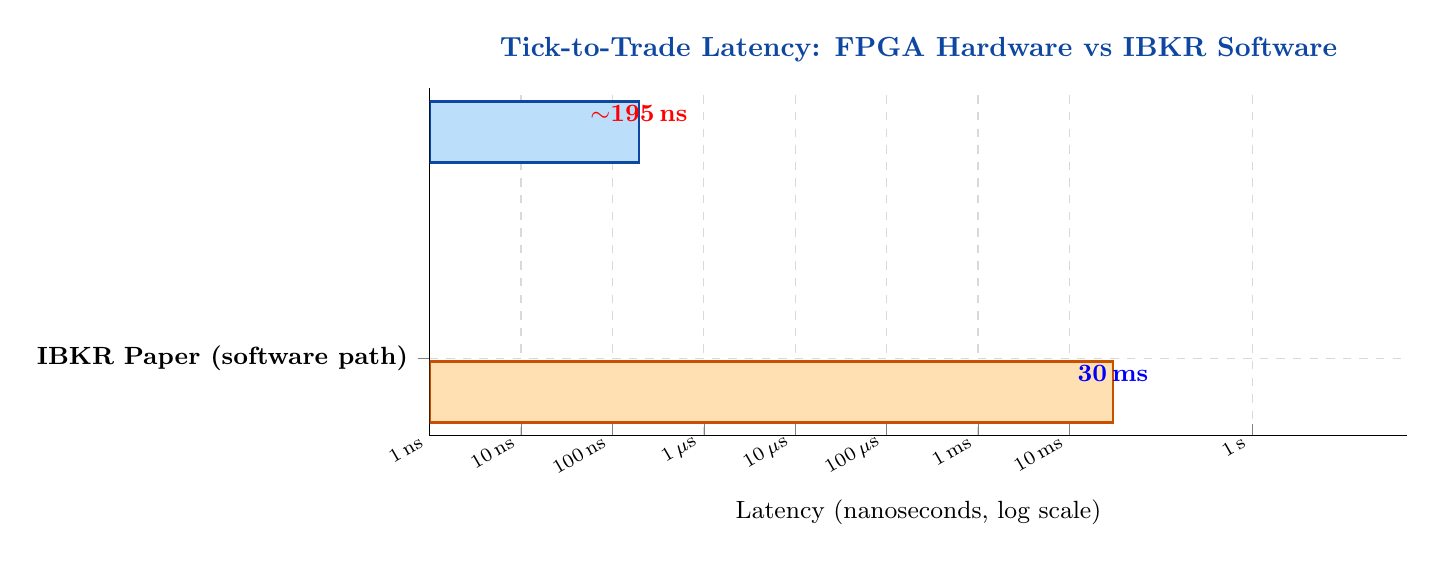
\begin{tikzpicture}
\begin{axis}[
  xbar, xmode=log,
  width=14cm, height=6cm,
  bar width=22pt,
  xlabel={Latency (nanoseconds, log scale)},
  xlabel style={font=\small},
  symbolic y coords={IBKR Paper (software path), FPGA Pipeline (hardware)},
  ytick=data,
  yticklabel style={font=\small\bfseries},
  xmin=1, xmax=5e10,
  xtick={1,10,100,1000,10000,100000,1000000,10000000,1000000000},
  xticklabels={1\,ns,10\,ns,100\,ns,1\,$\mu$s,10\,$\mu$s,100\,$\mu$s,1\,ms,10\,ms,1\,s},
  xticklabel style={font=\scriptsize, rotate=30, anchor=east},
  nodes near coords,
  nodes near coords align={horizontal},
  every node near coord/.append style={font=\small\bfseries},
  point meta=explicit symbolic,
  axis x line*=bottom,
  axis y line*=left,
  grid=major, grid style={dashed, gray!30},
  title={\bfseries Tick-to-Trade Latency: FPGA Hardware vs IBKR Software},
  title style={font=\normalsize, color=fpgablue},
  enlarge y limits=0.4,
]
\addplot+[fill=ibkrlight, draw=ibkrorange, line width=1pt]
  coordinates {(30000000,{IBKR Paper (software path)}) [30\,ms]};
\addplot+[fill=fpgalight, draw=fpgablue, line width=1pt]
  coordinates {(195,{FPGA Pipeline (hardware)}) [$\sim$195\,ns]};
\end{axis}
\end{tikzpicture}
\end{center}

\noindent The FPGA is approximately \textbf{154{,}000$\times$ faster}
(195\,ns measured vs.\ 30\,ms).
The log scale is necessary — on a linear scale the FPGA bar would be invisible.
This single chart is the core portfolio artefact.

\subsection{FPGA Determinism vs CPU Jitter}

\begin{center}
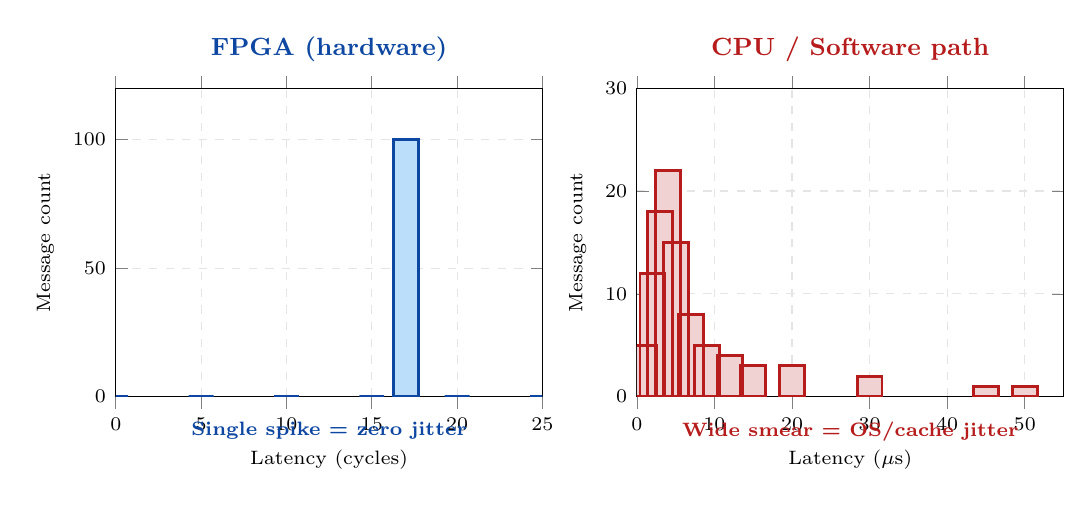
\begin{tikzpicture}
  \begin{axis}[
    name=axleft,
    ybar, width=7cm, height=5.5cm, bar width=9pt,
    xlabel={\scriptsize Latency (cycles)},
    ylabel={\scriptsize Message count},
    xlabel style={font=\scriptsize},
    ylabel style={font=\scriptsize},
    xticklabel style={font=\scriptsize},
    yticklabel style={font=\scriptsize},
    xmin=0, xmax=25, ymin=0, ymax=120,
    xtick={0,5,10,15,20,25},
    title={\small\bfseries FPGA (hardware)},
    title style={color=fpgablue, font=\small},
    grid=major, grid style={dashed, gray!20},
  ]
  \addplot[fill=fpgalight, draw=fpgablue, line width=1pt] coordinates {
    (0,0)(5,0)(10,0)(15,0)(17,100)(20,0)(25,0)
  };
  \end{axis}

  \begin{axis}[
    name=axright,
    at={(axleft.east)}, anchor=west, xshift=1.2cm,
    ybar, width=7cm, height=5.5cm, bar width=9pt,
    xlabel={\scriptsize Latency ($\mu$s)},
    ylabel={\scriptsize Message count},
    xlabel style={font=\scriptsize},
    ylabel style={font=\scriptsize},
    xticklabel style={font=\scriptsize},
    yticklabel style={font=\scriptsize},
    xmin=0, xmax=55, ymin=0, ymax=30,
    xtick={0,10,20,30,40,50},
    title={\small\bfseries CPU / Software path},
    title style={color=sigred, font=\small},
    grid=major, grid style={dashed, gray!20},
  ]
  \addplot[fill=sigred!20, draw=sigred, line width=1pt] coordinates {
    (1,5)(2,12)(3,18)(4,22)(5,15)(7,8)(9,5)(12,4)(15,3)(20,3)(30,2)(45,1)(50,1)
  };
  \end{axis}

  % Labels
  \node[font=\scriptsize\bfseries, fpgablue, below=0.2cm of axleft.south]
    {Single spike = zero jitter};
  \node[font=\scriptsize\bfseries, sigred, below=0.2cm of axright.south]
    {Wide smear = OS/cache jitter};
\end{tikzpicture}
\end{center}

% ─────────────────────────────────────────────────────────────────────────────
\section{Milestone Checklist}

\begin{center}
\small
\begin{tabular}{l p{5cm} l}
\toprule
\textbf{Milestone} & \textbf{Deliverable} & \textbf{Status} \\
\midrule
\cmark & \texttt{itch\_parser.sv}: 11/11 tests, 8 ITCH message types & Done \\
\cmark & \texttt{order\_book\_top.sv}: 11/11 tests vs golden model & Done \\
\cmark & \texttt{order\_book\_m2.sv}: 28/28 tests, multi-level + RESCAN & Done \\
\cmark & \texttt{strategy\_imbalance.sv}: 21/21 tests, depth-weighted & Done \\
\cmark & \texttt{latency\_counter.sv}: 5/5 tests, AXI-Lite readout & Done \\
\cmark & Integration test (\texttt{tick\_to\_trade\_top}): 5/5, \textbf{195\,ns} measured & Done \\
\cmark & \texttt{order\_book\_m2} wired into top-level; \texttt{msg\_ready} backpressure & Done \\
\cmark & Host: IBKR dry-run (\texttt{python ibkr\_bridge.py --demo}) & Done \\
\cmark & Jupyter latency dashboard (4 charts) & Done \\
\pmark & Vivado synthesis / timing closure on VU9P (larger-RAM machine) & Next \\
\pmark & Host: PCIe DMA read path; paper order visible in TWS & Pending \\
\pmark & AWS F1: AFI bitstream + hardware latency histogram & Pending \\
\pmark & LinkedIn post: numbers + chart + GitHub repo link & Pending \\
\bottomrule
\end{tabular}
\end{center}

% ─────────────────────────────────────────────────────────────────────────────
\section{Milestone 2 Scope}

\begin{center}
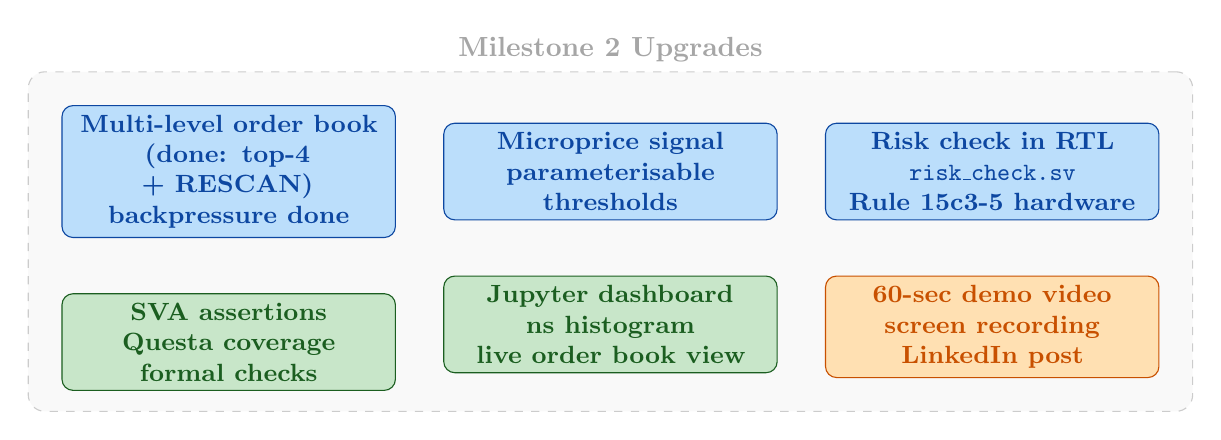
\begin{tikzpicture}[node distance=0.4cm and 0.6cm, font=\small]
  \node[fpgablock, minimum width=4.2cm, text width=4.0cm]
    (book2) {Multi-level order book\\\textbf{(done: top-4 + RESCAN)}\\backpressure done};
  \node[fpgablock, right=0.6cm of book2, minimum width=4.2cm, text width=4.0cm]
    (strat2) {Microprice signal\\parameterisable\\thresholds};
  \node[fpgablock, right=0.6cm of strat2, minimum width=4.2cm, text width=4.0cm]
    (risk2) {Risk check in RTL\\\texttt{risk\_check.sv}\\Rule 15c3-5 hardware};
  \node[hostblock, below=0.7cm of book2, minimum width=4.2cm, text width=4.0cm]
    (cov) {SVA assertions\\Questa coverage\\formal checks};
  \node[hostblock, below=0.7cm of strat2, minimum width=4.2cm, text width=4.0cm]
    (dash) {Jupyter dashboard\\ns histogram\\live order book view};
  \node[ibkrblock, below=0.7cm of risk2, minimum width=4.2cm, text width=4.0cm]
    (vid) {60-sec demo video\\screen recording\\LinkedIn post};

  \begin{scope}[on background layer]
    \node[dashbox, fill=gray!5, draw=gray!40,
          fit=(book2)(vid), inner sep=12pt,
          label={[gray!70, font=\bfseries]above:Milestone 2 Upgrades}] {};
  \end{scope}
\end{tikzpicture}
\end{center}

% ─────────────────────────────────────────────────────────────────────────────
\section{LinkedIn Write-Up Template}

Once hardware latency numbers are in hand, post this:

\begin{center}
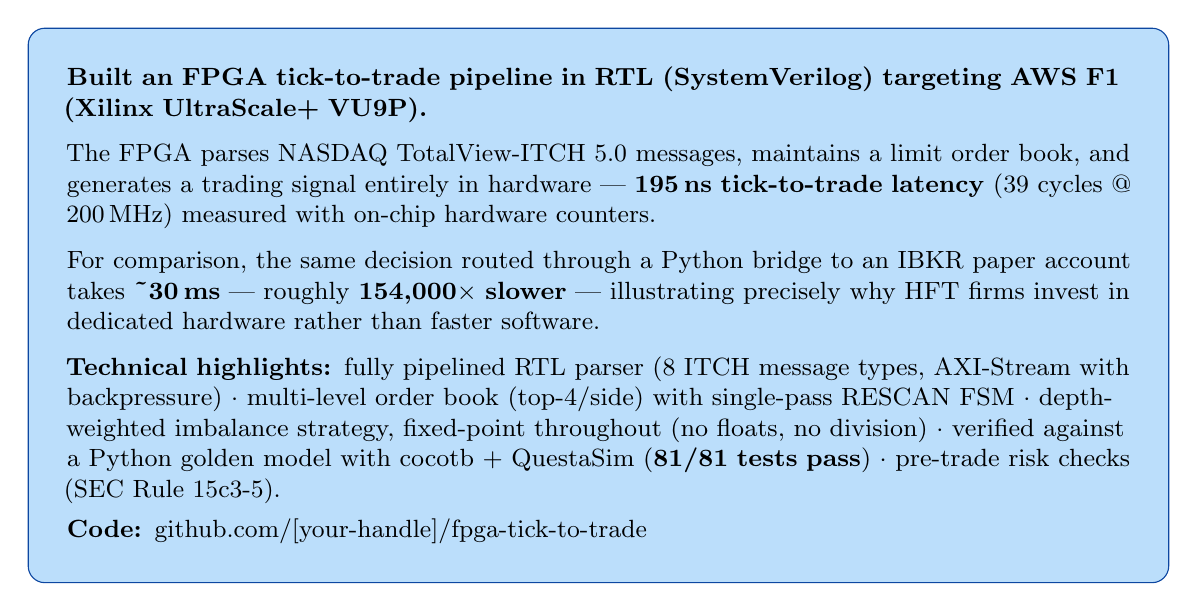
\begin{tikzpicture}
  \node[rectangle, rounded corners=6pt, fill=fpgalight, draw=fpgablue,
        text width=13.5cm, inner sep=14pt, font=\small] {
    \textbf{Built an FPGA tick-to-trade pipeline in RTL (SystemVerilog)
    targeting AWS F1 (Xilinx UltraScale+ VU9P).}\\[0.6em]
    The FPGA parses NASDAQ TotalView-ITCH 5.0 messages, maintains a limit
    order book, and generates a trading signal entirely in hardware ---
    \textbf{195\,ns tick-to-trade latency} (39 cycles @ 200\,MHz) measured with
    on-chip hardware counters.\\[0.6em]
    For comparison, the same decision routed through a Python bridge to an IBKR
    paper account takes \textbf{\textasciitilde{}30\,ms} --- roughly
    \textbf{154{,}000$\times$ slower} --- illustrating precisely why HFT firms
    invest in dedicated hardware rather than faster software.\\[0.6em]
    \textbf{Technical highlights:}
    fully pipelined RTL parser (8 ITCH message types, AXI-Stream with backpressure)
    $\cdot$ multi-level order book (top-4/side) with single-pass RESCAN FSM
    $\cdot$ depth-weighted imbalance strategy, fixed-point throughout (no floats, no division)
    $\cdot$ verified against a Python golden model with cocotb + QuestaSim
    (\textbf{81/81 tests pass}) $\cdot$ pre-trade risk checks (SEC Rule 15c3-5).\\[0.4em]
    \textbf{Code:} github.com/[your-handle]/fpga-tick-to-trade
  };
\end{tikzpicture}
\end{center}

\noindent\textbf{What not to claim:} Do not say ``nanosecond live trading
through IBKR'' — physically impossible. Do not claim the strategy is profitable
(it is a paper account with a simple imbalance signal). Do not imply
wire-to-wire latency unless the Ethernet path is fully in FPGA logic
(only true on F1 with a custom shell).

\end{document}
